% Options for packages loaded elsewhere
\PassOptionsToPackage{unicode}{hyperref}
\PassOptionsToPackage{hyphens}{url}
%
\documentclass[
]{book}
\usepackage{amsmath,amssymb}
\usepackage{lmodern}
\usepackage{iftex}
\ifPDFTeX
  \usepackage[T1]{fontenc}
  \usepackage[utf8]{inputenc}
  \usepackage{textcomp} % provide euro and other symbols
\else % if luatex or xetex
  \usepackage{unicode-math}
  \defaultfontfeatures{Scale=MatchLowercase}
  \defaultfontfeatures[\rmfamily]{Ligatures=TeX,Scale=1}
\fi
% Use upquote if available, for straight quotes in verbatim environments
\IfFileExists{upquote.sty}{\usepackage{upquote}}{}
\IfFileExists{microtype.sty}{% use microtype if available
  \usepackage[]{microtype}
  \UseMicrotypeSet[protrusion]{basicmath} % disable protrusion for tt fonts
}{}
\makeatletter
\@ifundefined{KOMAClassName}{% if non-KOMA class
  \IfFileExists{parskip.sty}{%
    \usepackage{parskip}
  }{% else
    \setlength{\parindent}{0pt}
    \setlength{\parskip}{6pt plus 2pt minus 1pt}}
}{% if KOMA class
  \KOMAoptions{parskip=half}}
\makeatother
\usepackage{xcolor}
\IfFileExists{xurl.sty}{\usepackage{xurl}}{} % add URL line breaks if available
\IfFileExists{bookmark.sty}{\usepackage{bookmark}}{\usepackage{hyperref}}
\hypersetup{
  pdftitle={Manipulating Time Series Data in R},
  pdfauthor={Harrison Brown},
  hidelinks,
  pdfcreator={LaTeX via pandoc}}
\urlstyle{same} % disable monospaced font for URLs
\usepackage{color}
\usepackage{fancyvrb}
\newcommand{\VerbBar}{|}
\newcommand{\VERB}{\Verb[commandchars=\\\{\}]}
\DefineVerbatimEnvironment{Highlighting}{Verbatim}{commandchars=\\\{\}}
% Add ',fontsize=\small' for more characters per line
\usepackage{framed}
\definecolor{shadecolor}{RGB}{248,248,248}
\newenvironment{Shaded}{\begin{snugshade}}{\end{snugshade}}
\newcommand{\AlertTok}[1]{\textcolor[rgb]{0.94,0.16,0.16}{#1}}
\newcommand{\AnnotationTok}[1]{\textcolor[rgb]{0.56,0.35,0.01}{\textbf{\textit{#1}}}}
\newcommand{\AttributeTok}[1]{\textcolor[rgb]{0.77,0.63,0.00}{#1}}
\newcommand{\BaseNTok}[1]{\textcolor[rgb]{0.00,0.00,0.81}{#1}}
\newcommand{\BuiltInTok}[1]{#1}
\newcommand{\CharTok}[1]{\textcolor[rgb]{0.31,0.60,0.02}{#1}}
\newcommand{\CommentTok}[1]{\textcolor[rgb]{0.56,0.35,0.01}{\textit{#1}}}
\newcommand{\CommentVarTok}[1]{\textcolor[rgb]{0.56,0.35,0.01}{\textbf{\textit{#1}}}}
\newcommand{\ConstantTok}[1]{\textcolor[rgb]{0.00,0.00,0.00}{#1}}
\newcommand{\ControlFlowTok}[1]{\textcolor[rgb]{0.13,0.29,0.53}{\textbf{#1}}}
\newcommand{\DataTypeTok}[1]{\textcolor[rgb]{0.13,0.29,0.53}{#1}}
\newcommand{\DecValTok}[1]{\textcolor[rgb]{0.00,0.00,0.81}{#1}}
\newcommand{\DocumentationTok}[1]{\textcolor[rgb]{0.56,0.35,0.01}{\textbf{\textit{#1}}}}
\newcommand{\ErrorTok}[1]{\textcolor[rgb]{0.64,0.00,0.00}{\textbf{#1}}}
\newcommand{\ExtensionTok}[1]{#1}
\newcommand{\FloatTok}[1]{\textcolor[rgb]{0.00,0.00,0.81}{#1}}
\newcommand{\FunctionTok}[1]{\textcolor[rgb]{0.00,0.00,0.00}{#1}}
\newcommand{\ImportTok}[1]{#1}
\newcommand{\InformationTok}[1]{\textcolor[rgb]{0.56,0.35,0.01}{\textbf{\textit{#1}}}}
\newcommand{\KeywordTok}[1]{\textcolor[rgb]{0.13,0.29,0.53}{\textbf{#1}}}
\newcommand{\NormalTok}[1]{#1}
\newcommand{\OperatorTok}[1]{\textcolor[rgb]{0.81,0.36,0.00}{\textbf{#1}}}
\newcommand{\OtherTok}[1]{\textcolor[rgb]{0.56,0.35,0.01}{#1}}
\newcommand{\PreprocessorTok}[1]{\textcolor[rgb]{0.56,0.35,0.01}{\textit{#1}}}
\newcommand{\RegionMarkerTok}[1]{#1}
\newcommand{\SpecialCharTok}[1]{\textcolor[rgb]{0.00,0.00,0.00}{#1}}
\newcommand{\SpecialStringTok}[1]{\textcolor[rgb]{0.31,0.60,0.02}{#1}}
\newcommand{\StringTok}[1]{\textcolor[rgb]{0.31,0.60,0.02}{#1}}
\newcommand{\VariableTok}[1]{\textcolor[rgb]{0.00,0.00,0.00}{#1}}
\newcommand{\VerbatimStringTok}[1]{\textcolor[rgb]{0.31,0.60,0.02}{#1}}
\newcommand{\WarningTok}[1]{\textcolor[rgb]{0.56,0.35,0.01}{\textbf{\textit{#1}}}}
\usepackage{longtable,booktabs,array}
\usepackage{calc} % for calculating minipage widths
% Correct order of tables after \paragraph or \subparagraph
\usepackage{etoolbox}
\makeatletter
\patchcmd\longtable{\par}{\if@noskipsec\mbox{}\fi\par}{}{}
\makeatother
% Allow footnotes in longtable head/foot
\IfFileExists{footnotehyper.sty}{\usepackage{footnotehyper}}{\usepackage{footnote}}
\makesavenoteenv{longtable}
\usepackage{graphicx}
\makeatletter
\def\maxwidth{\ifdim\Gin@nat@width>\linewidth\linewidth\else\Gin@nat@width\fi}
\def\maxheight{\ifdim\Gin@nat@height>\textheight\textheight\else\Gin@nat@height\fi}
\makeatother
% Scale images if necessary, so that they will not overflow the page
% margins by default, and it is still possible to overwrite the defaults
% using explicit options in \includegraphics[width, height, ...]{}
\setkeys{Gin}{width=\maxwidth,height=\maxheight,keepaspectratio}
% Set default figure placement to htbp
\makeatletter
\def\fps@figure{htbp}
\makeatother
\setlength{\emergencystretch}{3em} % prevent overfull lines
\providecommand{\tightlist}{%
  \setlength{\itemsep}{0pt}\setlength{\parskip}{0pt}}
\setcounter{secnumdepth}{5}
\usepackage{booktabs}
\ifLuaTeX
  \usepackage{selnolig}  % disable illegal ligatures
\fi
\usepackage[]{natbib}
\bibliographystyle{plainnat}

\title{Manipulating Time Series Data in R}
\author{Harrison Brown}
\date{2022-05-19}

\begin{document}
\maketitle

{
\setcounter{tocdepth}{1}
\tableofcontents
}
\hypertarget{welcome}{%
\chapter*{Welcome}\label{welcome}}
\addcontentsline{toc}{chapter}{Welcome}

Welcome to the course outline for \emph{Time Series Data in R}! This course offers methods and workflows for analyzing and interpreting time series data, an overview of when, why, and how to use time series data, and various utilities and packages in R that are beneficial to analysts.

By the end of this course, students will have the skills to:

\begin{itemize}
\tightlist
\item
  Interpret and understand time series plots
\item
  Import ts data to create and manipulate \texttt{ts} objects from the \texttt{stats} package
\item
  Understand why time series data is fundamentally different than non-ts data.
\item
  Analyze time series data with plots
\item
  ?Intro to Wavelet analysis?
\end{itemize}

\hypertarget{introduction-to-time-series-data}{%
\chapter{Introduction to time series data}\label{introduction-to-time-series-data}}

\hypertarget{lesson-what-is-time-series-data}{%
\section{Lesson: What is Time Series Data}\label{lesson-what-is-time-series-data}}

\begin{itemize}
\tightlist
\item
  Learning Objective: Learner will be able to understand why and how TS-data differs from non-temporal data
\item
  LO: What kinds of inferences and results can be obtained from TS-data
\item
  LO: Converting to and from time-based data formats, such as \texttt{numeric}, \texttt{Date}, and \texttt{POSIXct} classes

  \begin{itemize}
  \tightlist
  \item
    Functions: \texttt{as.Date()}, \texttt{lubridate::}, etc.
  \end{itemize}
\end{itemize}

\hypertarget{lesson-how-to-interpret-time-series-data}{%
\section{Lesson: How to Interpret Time Series Data}\label{lesson-how-to-interpret-time-series-data}}

\begin{itemize}
\tightlist
\item
  LO: Learner will understand how to interpret attributes of a basic time series plot
\item
  LO: ``Signal and Noise'' in the context of TS data
\item
  Introduction to Stationarity: Most real-world data are not stationary and require additional steps to work with
\end{itemize}

\hypertarget{lesson-components-of-time-series-data}{%
\section{Lesson: Components of Time Series Data}\label{lesson-components-of-time-series-data}}

\hypertarget{creating-and-manipulating-time-series}{%
\chapter{Creating and Manipulating Time Series}\label{creating-and-manipulating-time-series}}

\hypertarget{ts-class}{%
\section{\texorpdfstring{\texttt{ts} Class}{ts Class}}\label{ts-class}}

\hypertarget{missing-values}{%
\section{Missing Values}\label{missing-values}}

\begin{Shaded}
\begin{Highlighting}[]
\NormalTok{d }\OtherTok{\textless{}{-}} \FunctionTok{c}\NormalTok{(}\StringTok{\textquotesingle{}2001{-}01{-}01\textquotesingle{}}\NormalTok{, }\StringTok{\textquotesingle{}2001{-}01{-}02\textquotesingle{}}\NormalTok{, }\StringTok{\textquotesingle{}2001{-}01{-}04\textquotesingle{}}\NormalTok{, }\StringTok{\textquotesingle{}2001{-}01{-}05\textquotesingle{}}\NormalTok{)}
\NormalTok{d }\OtherTok{\textless{}{-}} \FunctionTok{as.Date}\NormalTok{(d)}
\NormalTok{date\_range }\OtherTok{\textless{}{-}} \FunctionTok{seq}\NormalTok{(}\FunctionTok{min}\NormalTok{(d), }\FunctionTok{max}\NormalTok{(d), }\AttributeTok{by =} \DecValTok{1}\NormalTok{) }
\NormalTok{date\_range[}\SpecialCharTok{!}\NormalTok{date\_range }\SpecialCharTok{\%in\%}\NormalTok{ d] }
\end{Highlighting}
\end{Shaded}

\begin{verbatim}
## [1] "2001-01-03"
\end{verbatim}

\hypertarget{rolling-and-expanding-windows}{%
\chapter{Rolling and Expanding Windows}\label{rolling-and-expanding-windows}}

\hypertarget{rolling-window}{%
\section{Rolling Window}\label{rolling-window}}

\begin{itemize}
\tightlist
\item
  Moving lower and upper bound
\end{itemize}

\hypertarget{data}{%
\subsection{Data}\label{data}}

\hypertarget{calculating-a-rolling-window}{%
\subsection{Calculating a Rolling Window}\label{calculating-a-rolling-window}}

\hypertarget{introduction-to-forecasting-in-r}{%
\chapter{Introduction to Forecasting in R}\label{introduction-to-forecasting-in-r}}

\hypertarget{methods-for-forecasting}{%
\section{Methods for Forecasting}\label{methods-for-forecasting}}

\hypertarget{exponential-smoothing}{%
\subsection{Exponential Smoothing}\label{exponential-smoothing}}

\hypertarget{capstone-exercise}{%
\chapter{Capstone Exercise}\label{capstone-exercise}}

The final exercise for this course involves performing a time series analysis on real-world data: Carbon Dioxide concentration at the Mauna Loa Observatory, from early 1959 to Present. You'll go through the process of imputing missing values, testing for stationarity, decomposing the time series, and adjusting for seasonality. The goal for this exercise is a plot showing the seasonal-adjusted time series, which shows the ``overall trend'' in the data over the last few decades.

\hypertarget{importing-the-data}{%
\section{Importing the Data}\label{importing-the-data}}

\begin{Shaded}
\begin{Highlighting}[]
\CommentTok{\# The following libraries are included for you}

\FunctionTok{library}\NormalTok{(tidyverse)}
\FunctionTok{library}\NormalTok{(zoo)}
\FunctionTok{library}\NormalTok{(forecast)}
\FunctionTok{library}\NormalTok{(tseries)}
\CommentTok{\# Sample data from the Mauna Loa Observatory}
\CommentTok{\# https://gml.noaa.gov/webdata/ccgg/trends/co2/co2\_mm\_mlo.csv}

\CommentTok{\# Data is already pre{-}processed as a \textasciigrave{}ts\textasciigrave{} object. It contains missing values, so}
\CommentTok{\# we\textquotesingle{}ll need to impute those!}
\NormalTok{co2 }\OtherTok{\textless{}{-}} \FunctionTok{readRDS}\NormalTok{(}\StringTok{"data/missing.Rds"}\NormalTok{)}
\end{Highlighting}
\end{Shaded}

\hypertarget{visual-checks}{%
\section{Visual Checks}\label{visual-checks}}

\begin{enumerate}
\def\labelenumi{\arabic{enumi}.}
\tightlist
\item
  Plot your co2 data and see if the data is stationary, non-stationary (time-dependent), and seasonal or non-seasonal. Use the Augmented Dickey-Fuller test to determine stationarity.
\end{enumerate}

\begin{Shaded}
\begin{Highlighting}[]
\FunctionTok{plot.ts}\NormalTok{(co2)}
\end{Highlighting}
\end{Shaded}

\begin{center}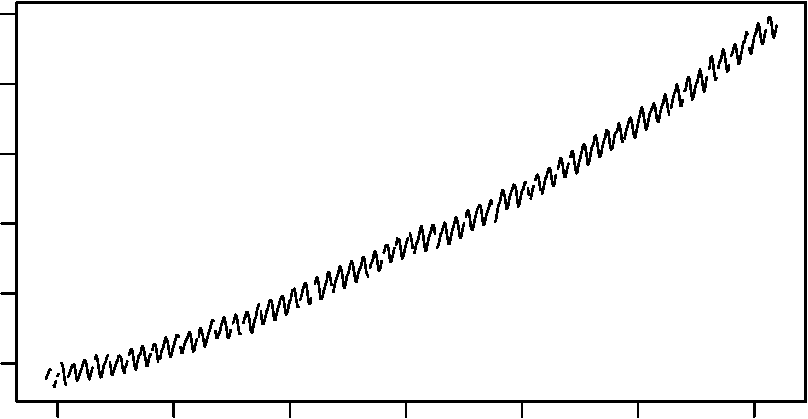
\includegraphics{_main_files/figure-latex/visual-1} \end{center}

\begin{Shaded}
\begin{Highlighting}[]
\FunctionTok{adf.test}\NormalTok{(co2)}
\end{Highlighting}
\end{Shaded}

\begin{verbatim}
## Error in adf.test(co2): NAs in x
\end{verbatim}

Looks like we have some missing values! Let's try and impute those to fill in the gaps:

\begin{enumerate}
\def\labelenumi{\arabic{enumi}.}
\setcounter{enumi}{1}
\tightlist
\item
  Impute missing values with the \texttt{na.approx()} function from \texttt{zoo}:
\end{enumerate}

\begin{Shaded}
\begin{Highlighting}[]
\NormalTok{co2 }\OtherTok{\textless{}{-}}\NormalTok{ co2 }\SpecialCharTok{\%\textgreater{}\%} 
\NormalTok{  zoo}\SpecialCharTok{::}\FunctionTok{na.approx}\NormalTok{()}

\FunctionTok{adf.test}\NormalTok{(co2)}
\end{Highlighting}
\end{Shaded}

\begin{verbatim}
## Warning in adf.test(co2): p-value greater than printed p-value
\end{verbatim}

\begin{verbatim}
## 
##  Augmented Dickey-Fuller Test
## 
## data:  co2
## Dickey-Fuller = -0.12404, Lag order = 9, p-value = 0.99
## alternative hypothesis: stationary
\end{verbatim}

Based on the statistic and p-value, the data is non-stationary.

\hypertarget{decomposing-the-time-series}{%
\section{Decomposing the Time Series}\label{decomposing-the-time-series}}

We're interested in the seasonal, remainder, and specifically, trend components. We want to know what the data looks like when adjusted for seasonality. To do this, we need to decompose our time series into its ETS components. Then, we can remove the seasonal component.

\begin{enumerate}
\def\labelenumi{\arabic{enumi}.}
\setcounter{enumi}{2}
\tightlist
\item
  Decompose the time series and plot the resulting \texttt{decomposed.ts} object:
\end{enumerate}

\begin{Shaded}
\begin{Highlighting}[]
\NormalTok{co2\_decomp }\OtherTok{\textless{}{-}}\NormalTok{ co2 }\SpecialCharTok{\%\textgreater{}\%}
  \FunctionTok{decompose}\NormalTok{()}

\FunctionTok{plot}\NormalTok{(co2\_decomp)}
\end{Highlighting}
\end{Shaded}

\begin{center}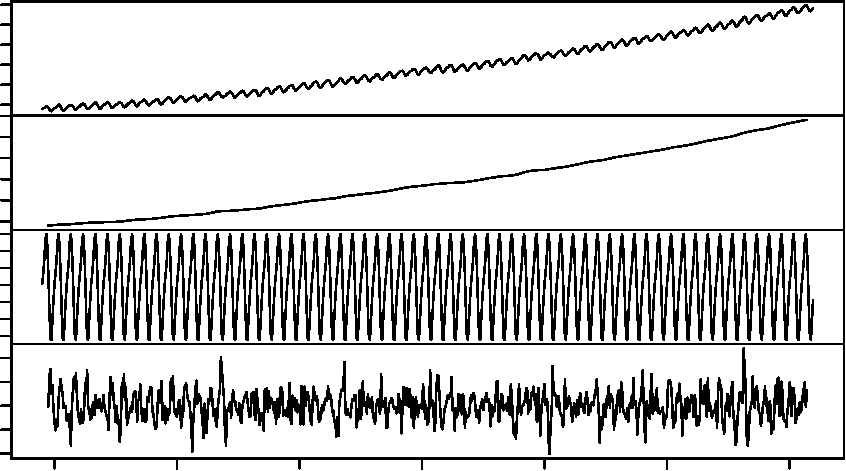
\includegraphics{_main_files/figure-latex/decomp-1} \end{center}

\begin{enumerate}
\def\labelenumi{\arabic{enumi}.}
\setcounter{enumi}{3}
\tightlist
\item
  Then, adjust for seasonality, and plot the results. Label the y-axis as ``CO2 Concentration'', and title the plot ``Seasonally-adjusted CO2 Concentration'':
\end{enumerate}

\begin{Shaded}
\begin{Highlighting}[]
\NormalTok{co2\_decomp }\SpecialCharTok{\%\textgreater{}\%} 
  \FunctionTok{seasadj}\NormalTok{() }\SpecialCharTok{\%\textgreater{}\%} 
  
  \CommentTok{\# If we want to include a rolling window, it\textquotesingle{}s really easy to do with}
  \CommentTok{\# zoo::rollapplyr()}
  
  \CommentTok{\#rollapplyr(FUN = mean, width = 12) \%\textgreater{}\%}
  \FunctionTok{plot}\NormalTok{(}\AttributeTok{ylab =} \StringTok{"CO2 Concentration"}\NormalTok{, }\AttributeTok{main =} \StringTok{"Seasonally{-}adjusted CO2 Concentration"}\NormalTok{)}
\end{Highlighting}
\end{Shaded}

\begin{center}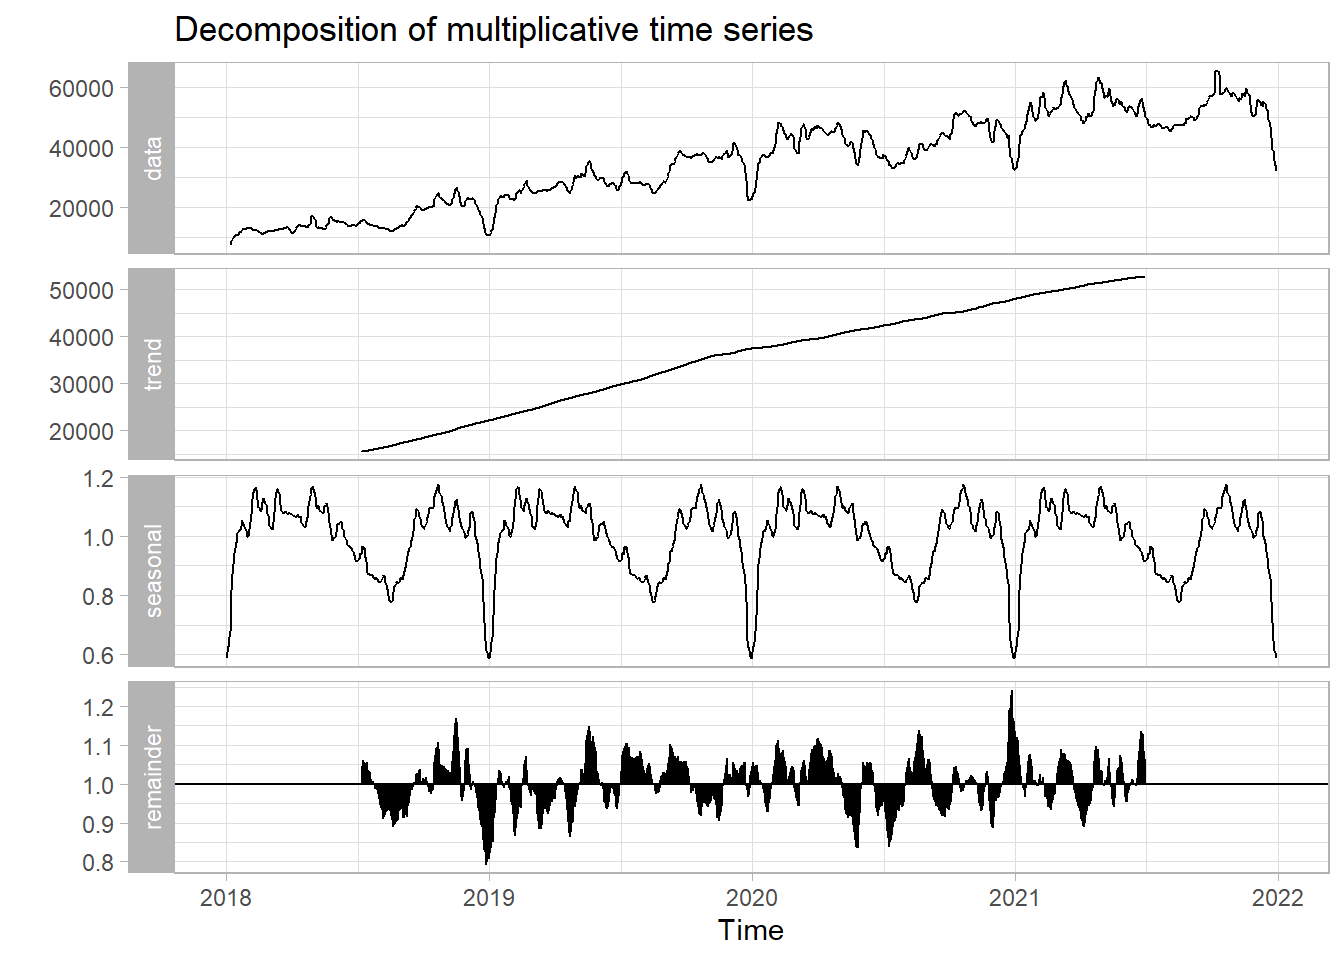
\includegraphics{_main_files/figure-latex/unnamed-chunk-7-1} \end{center}

Voila! We now have the overall trend, plus remainder component, of CO2 concentrations. By removing the seasonality of data, we can better assess the year-to-year differences in our data, and can reduce the effect of intra- and inter-year cycles present in the data.

\hypertarget{example-code}{%
\section{Example Code}\label{example-code}}

This is the code given in the exercise itself

Step 1:

\begin{Shaded}
\begin{Highlighting}[]
\FunctionTok{plot}\NormalTok{(\_\_\_)}

\FunctionTok{\_\_\_.test}\NormalTok{(co2)}
\end{Highlighting}
\end{Shaded}

Step 2:

\begin{Shaded}
\begin{Highlighting}[]
\NormalTok{co2\_impute }\OtherTok{\textless{}{-}}\NormalTok{ co2 }\SpecialCharTok{\%\textgreater{}\%} 
  \FunctionTok{\_\_.\_\_\_}\NormalTok{()}

\FunctionTok{adf.test}\NormalTok{(co2\_impute)}
\end{Highlighting}
\end{Shaded}

Step 3:

\begin{Shaded}
\begin{Highlighting}[]
\NormalTok{co2\_decomp }\OtherTok{\textless{}{-}}\NormalTok{ co2\_impute }\SpecialCharTok{\%\textgreater{}\%} 
  \FunctionTok{\_\_\_}\NormalTok{()}

\FunctionTok{plot}\NormalTok{(\_\_\_)}
\end{Highlighting}
\end{Shaded}

Step 4:

\begin{Shaded}
\begin{Highlighting}[]
\NormalTok{co2\_decomp }\SpecialCharTok{\%\textgreater{}\%} 
  \FunctionTok{\_\_\_\_}\NormalTok{() }\SpecialCharTok{\%\textgreater{}\%} 
  \FunctionTok{plot}\NormalTok{(}\AttributeTok{ylab =} \StringTok{"\_\_\_"}\NormalTok{, }\AttributeTok{main =} \StringTok{"\_\_\_"}\NormalTok{)}
\end{Highlighting}
\end{Shaded}

\hypertarget{course-outline-manipulating-time-series-data-in-r}{%
\chapter{Course Outline: Manipulating Time Series Data in R}\label{course-outline-manipulating-time-series-data-in-r}}

\emph{This course will introduce learners to working with time series data in R. Learners will explore how to store and format data in date and time objects as well as how to manipulate time series datasets through subsetting, indexing, and extraction. Examples of time series data across a variety of fields in business and science should be discussed. The course will cover summarization, frequency, missing data, resampling, and comparison techniques as well as window functions for both rolling and expanding windows.}

Packages Used:

\begin{itemize}
\tightlist
\item
  \texttt{base} and \texttt{stats} (default libraries, but I wanted to name them explicitly)
\item
  \texttt{zoo}
\end{itemize}

\begin{center}\rule{0.5\linewidth}{0.5pt}\end{center}

\hypertarget{chapter-1-introduction-to-time-series-data}{%
\section{Chapter 1: Introduction to Time Series Data}\label{chapter-1-introduction-to-time-series-data}}

\begin{itemize}
\tightlist
\item
  Lesson 1.1: \emph{What is Time Series Data}

  \begin{itemize}
  \tightlist
  \item
    LO: Learner will be able to understand the foundations of time series data: rather than just analyzing a variable at different points in time, ts analysis studies \emph{how} that variable changes with time.
  \end{itemize}
\item
  Lesson 1.2: \emph{Interpreting a Time Series}

  \begin{itemize}
  \tightlist
  \item
    LO: Learner will be able to interpret a time series graph, understanding the x- and y-axes, trend, identifying periods, etc. at an introductory level.
  \end{itemize}
\item
  Lesson 1.3: \emph{Temporal data classes in R}

  \begin{itemize}
  \tightlist
  \item
    LO: Introduction to different formats for temporal data in R, such as the \texttt{Date}, \texttt{numeric}, and \texttt{character} formats:

    \begin{itemize}
    \tightlist
    \item
      e.g.: 2022-01-30, \texttt{19022}, and ``2022-01-30'' share the same information, but in different formats
    \end{itemize}
  \item
    LO: Learners will be able to check classes of data stored as vectors or as columns in a dataframe or tibble.

    \begin{itemize}
    \tightlist
    \item
      \texttt{class()}
    \end{itemize}
  \end{itemize}
\item
  Lesson 1.4: \emph{Converting between data classes}

  \begin{itemize}
  \tightlist
  \item
    LO: Learners will be able to convert between classes in R, such as converting a \texttt{character} vector to a \texttt{Date} vector

    \begin{itemize}
    \tightlist
    \item
      \texttt{as.Date()}
    \item
      \texttt{as.numeric()}
    \item
      \texttt{as.character()}
    \end{itemize}
  \end{itemize}
\end{itemize}

\begin{center}\rule{0.5\linewidth}{0.5pt}\end{center}

\hypertarget{chapter-2-time-series-objects-in-r}{%
\section{Chapter 2: Time Series objects in R}\label{chapter-2-time-series-objects-in-r}}

\begin{itemize}
\tightlist
\item
  Lesson 2.1: \emph{How does R store Time Series Data?}

  \begin{itemize}
  \tightlist
  \item
    LO: Learners will be introduced to \texttt{ts} objects in R, and how they differ from objects like vectors or data frames
  \item
    LO: Retrieve the temporal attributes (start, end, and frequency) of a time series object.

    \begin{itemize}
    \tightlist
    \item
      \texttt{start()}
    \item
      \texttt{end()}
    \item
      \texttt{frequency()}
    \end{itemize}
  \end{itemize}
\item
  Lesson 2.2: \emph{Create a Time Series object in Base R}

  \begin{itemize}
  \tightlist
  \item
    LO: Convert a vector of observations into a \texttt{ts} object, specifying start time and frequency

    \begin{itemize}
    \tightlist
    \item
      \texttt{ts()}
    \end{itemize}
  \end{itemize}
\item
  Lesson 2.3: \emph{Using the Zoo Package to store time series data}

  \begin{itemize}
  \tightlist
  \item
    LO: What is \texttt{zoo} and why is it different from base \texttt{ts}?

    \begin{itemize}
    \tightlist
    \item
      Zoo can use irregular time intervals
    \end{itemize}
  \item
    LO: Create and coerce time series objects with the \texttt{zoo} package:

    \begin{itemize}
    \tightlist
    \item
      \texttt{zoo::zoo()}
    \item
      \texttt{zoo::as.zoo()}
    \end{itemize}
  \end{itemize}
\item
  Lesson 2.4: \emph{Using Zoo to extract time and data vectors}

  \begin{itemize}
  \tightlist
  \item
    LO: Extract ``core data'' and time data from a \texttt{ts} or \texttt{zoo} object:

    \begin{itemize}
    \tightlist
    \item
      \texttt{time()}
    \item
      \texttt{zoo::coredata()}
    \end{itemize}
  \end{itemize}
\end{itemize}

\begin{center}\rule{0.5\linewidth}{0.5pt}\end{center}

\hypertarget{chapter-3-subsetting-extracting-and-resampling}{%
\section{Chapter 3: Subsetting, Extracting, and Resampling}\label{chapter-3-subsetting-extracting-and-resampling}}

\begin{itemize}
\tightlist
\item
  Lesson 3.1: \emph{Subsetting a window of observations}

  \begin{itemize}
  \tightlist
  \item
    LO: Learner will be able to extract a window of observations between a set of time intervals

    \begin{itemize}
    \tightlist
    \item
      \texttt{window()}
    \item
      \texttt{as.Date()}
    \item
      \texttt{zoo::as.yearmon()}
    \end{itemize}
  \item
    LO: Use the \texttt{\textquotesingle{}{[}\textquotesingle{}} operator with \texttt{as.Date()} to extract a specific date's observation

    \begin{itemize}
    \tightlist
    \item
      \texttt{\textquotesingle{}{[}\textquotesingle{}}
    \item
      \texttt{as.Date()}
    \item
      \texttt{zoo::as.yearmon()}
    \end{itemize}
  \end{itemize}
\item
  Lesson 3.2: \emph{Retrieving observations by index}

  \begin{itemize}
  \tightlist
  \item
    LO: Use standard R \texttt{\textquotesingle{}{[}\textquotesingle{}} operator to extract one or more observations by numerical index

    \begin{itemize}
    \tightlist
    \item
      \texttt{\textquotesingle{}{[}\textquotesingle{}}
    \item
      e.g.: \texttt{data{[}1:20{]}} retrieves observations 1 through 20
    \end{itemize}
  \end{itemize}
\item
  Lesson 3.3: \emph{Resampling observations}

  \begin{itemize}
  \tightlist
  \item
    LO: Learner will be able to resample observations to any interval of time (yearly, monthly, quarterly, etc.)

    \begin{itemize}
    \tightlist
    \item
      \texttt{aggregate()}
    \item
      e.g.: \texttt{aggregate(data,\ nfrequency\ =\ 12,\ FUN\ =\ sum)} finds sums of observations within each month.
    \end{itemize}
  \end{itemize}
\item
  Lesson 3.4: \emph{Imputing Missing Values}

  \begin{itemize}
  \tightlist
  \item
    LO: Use the \texttt{zoo} package to impute missing values with either linear interpolation or cubic spline interpolation

    \begin{itemize}
    \tightlist
    \item
      \texttt{zoo::na.approx()} and \texttt{zoo::na.spline()}, respectively
    \end{itemize}
  \end{itemize}
\end{itemize}

\begin{center}\rule{0.5\linewidth}{0.5pt}\end{center}

\hypertarget{chapter-4-rolling-and-expanding-windows}{%
\section{Chapter 4: Rolling and Expanding Windows}\label{chapter-4-rolling-and-expanding-windows}}

\begin{itemize}
\tightlist
\item
  Lesson 4.1: \emph{What are windows?}

  \begin{itemize}
  \tightlist
  \item
    LO: Learner will understand the utility of rolling and expanding windows: finding moving averages, cumulative sums, etc.
  \end{itemize}
\item
  Lesson 4.2: \emph{Calculating a Rolling Window}

  \begin{itemize}
  \tightlist
  \item
    LO: Learner will be able to perform a rolling window operation on a time series, creating a moving average (or moving sum) of any length

    \begin{itemize}
    \tightlist
    \item
      \texttt{zoo::rollapply()}
    \item
      \texttt{zoo::rollapplyr()} (convenience wrapper for \texttt{zoo::rollapply(align\ =\ "right")})
    \item
      e.g.: \texttt{zoo::rollapplyr(daily\_data,\ FUN\ =\ mean,\ width\ =\ 7)} to create a 7-day rolling average from \texttt{daily\_data}
    \end{itemize}
  \end{itemize}
\item
  Lesson 4.3: \emph{Calculating an Expanding Window}

  \begin{itemize}
  \tightlist
  \item
    LO: Learner will be able to create an expanding window: a rolling window where the ``start'' is fixed and the ``end'' moves

    \begin{itemize}
    \tightlist
    \item
      \texttt{cumsum()}
    \item
      \texttt{seq\_along()}
    \item
      e.g.: \texttt{cumsum(x)\ /\ seq\_along(x)} calculates a cumulative mean
    \item
      \emph{this function exists in \texttt{dplyr::cummean()}, but I didn't want an entire package dependency for something so simple}
    \end{itemize}
  \end{itemize}
\item
  Lesson 4.4: \emph{Plotting windows alongside Data}

  \begin{itemize}
  \tightlist
  \item
    LO: Learner will be able to plot the rolling/expanding window alongside the original data, in order to visually assess how these operations affect the data

    \begin{itemize}
    \tightlist
    \item
      \texttt{plot()}
    \item
      \texttt{lines()}
    \end{itemize}
  \end{itemize}
\end{itemize}

  \bibliography{book.bib,packages.bib}

\end{document}
